%%%%%%%%%%%%%%%%%%%%% chapter.tex %%%%%%%%%%%%%%%%%%%%%%%%%%%%%%%%%
%
% sample chapter
%
% Use this file as a template for your own input.
%
%%%%%%%%%%%%%%%%%%%%%%%% Springer-Verlag %%%%%%%%%%%%%%%%%%%%%%%%%%
%\motto{Use the template \emph{chapter.tex} to style the various elements of your chapter content.}
\chapter{人脸识别}
\label{basic} % Always give a unique label
% use \chaptermark{}
% to alter or adjust the chapter heading in the running head


\section{问题定义}
人脸识别,是指对输入的图像和视频,检测其中存在的人脸,依据人脸的面部特征,完成身份识别的过程,属于生物特征识别技术。整个流程包含人脸检测、人脸对齐、人脸特征提取、人脸匹配几个阶段,如图 \ref{fig:face_recog_flow_chart} 所示。目前人脸识别已经广泛应用于安防、金融、军事等领域。

人脸识别具有以下优点:

自然性:所谓自然性,是指人脸识别技术所利用的生物特征,与人类进行人脸识别时所利用的生物特征是一致的,与之相比,虹膜识别、指纹识别等技术,则不具备自然性。

非接触性:在人脸识别技术中,用户不会与识别设备发生任何接触,对于用户来说体验较好。而指纹识别则需要用户进行按压设备。

使用便捷:用户使用人脸识别技术时非常方便,基本上无需做特殊的配合。

人脸识别也具有一些缺点,比如易受光照条件的影响,易受人脸遮挡物的影响,跨年龄识别难度较高等。但总的来说,人脸识别是目前一种可靠的,实用的,便捷的身份核验技术。

\begin{figure}[ht]
\centering
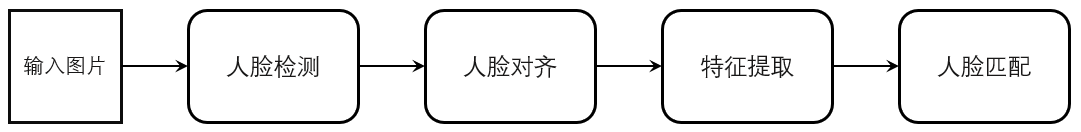
\includegraphics[scale=0.5]{img/chapter_fr/face_recog_flow_chart.png}
\caption{人脸识别流程图}
\label{fig:face_recog_flow_chart}
\end{figure}

\section{实现方案}
\subsection{人脸检测及对齐}
人脸检测是人脸识别的第一步,属于目标检测的子方向。其目的是找出图像中的人脸以及对应的位置。可能还会包含一些人脸的额外信息,比如人脸的关键点,姿态角度等。

典型的人脸检测是基于以下的流程:由于人脸可能出现的图像的任何位置,因此需要通过滑动窗口(sliding windows)来获取可能包含人脸的子图像。获取到的子图像,需要通过一个二分类的分类器,来判断图像中是否包含人脸,如果还需要确定人脸的精确位置,还需要加上一个回归人脸框的操作。同一个人脸可能会检测出多个人脸框,因此需要使用非极大值抑制(Non-Maximum suppression, NMS)来进行合并去重。由于人脸有大有小,为了更好的检测出不同尺度的人脸,还需要输入图像做不同尺度的图像缩放,也叫图像金字塔技术。接下来本文介绍一些具有代表性的人脸检测方法。

Viola-jones\cite{viola2001rapid}是2001年提出的一个人脸检测方法,该方法具有检测效率高,并且能够保持较好的精度的特点,是第一个具有实用意义的人脸检测算法。该方法使用Haar-like小波特征,并通过级联的AdaBoost分类器构造检测器。同时,还是用了积分图来加速Haar-like输入特征的计算。这是一个具有里程碑意义的方法。

MTCNN\cite{zhang2016joint}是2016年提出的一个人脸检测方法,它将人脸分类、人脸框回归以及人脸关键点定位在同一个任务内完成了,是一个多任务(multi-task)的检测方法,这种思路在后续的很多方法里也得到了使用。该方法采用三级网络级联的方法,定义了3个子网络:P-Net,R-Net以及O-Net,P-Net用于快速产生候选框,使用全卷积运算代替了滑动窗口,大大提升效率,R-Net和O-Net用于对候选框进行精细调整。

anchor的思想在Faster-rcnn\cite{ren2015faster}中首先被提出,该方法被广泛应用于两阶段和单阶段的目标检测任务中,在人脸检测中也经常使用到。anchor提出的目的是为了解决目标在图像中可能以不同的形状存在,比如不同的长宽比,所以加入人工的先验信息,预先定义不同比例的anchor来进行候选目标框的获取。Face r-cnn\cite{wang2017face}, Pyramidbox\cite{tang2018pyramidbox}, Retinaface\cite{deng2019retinaface}这些方法,都用到了anchor的思想。另一个在人脸检测中经常使用的思想是特征金字塔网络(feature pyramid network),人脸在图像中,可能以不同尺度的大小出现,为了能够对大人脸和小人脸都有很好的检测效果,一般有两种做法,一种做法是图像金字塔,这种方法需要对输入图像做不同尺度的缩放,缺点是耗时较高;另一种更好的做法则是特征金字塔,其思想是在不同分辨率的特征图(feature map)上检测对应尺度的目标,同时将不同分辨率的特征图与更高层的特征图进行特征融合,保证每一层的特征图都具有足够的表达能力。Pyramidbox,Retinaface都用到了特征金字塔,SSH\cite{najibi2017ssh}虽然没有直接用到特征金字塔,但其也是对网络3个不同尺度的特征图进行分别预测,来解决多尺度的人脸检测问题。

人脸检测检测通常会以检测率、误检率等作为评估指标,同时会关注性能指标。很多算法的效果很好,但性能会很差,做不到实时,也就限制了使用场景。

做完人脸检测后,一般需要进行人脸对齐。通过对人脸进行关键点定位,以及预先定义好的关键点模板,进行仿射变换,通过旋转、平移、缩放等操作,进行人脸对齐,对齐后的人脸能够更好的进行人脸特征提取。目前常见的关键点个数,有5个关键点、68个关键点、90个关键点以及106个关键点等。

\subsection{人脸特征提取}
人脸识别中,最重要的步骤是人脸特征提取,将人脸在高维空间的描述转化为其他空间内的低维描述,使得转化后的特征能够很好地区分不同人之间的差异点。经过特征提取得到人脸的特征表示之后,可以进行特征匹配。如果是对两个特征进行比对,我们一般称为人脸比对或者人脸验证(verification),如果是将一个特征与一组特征进行匹配,我们一般称为人脸检索或者人脸识别(identification),如图 \ref{fig:verification_identification} 所示。匹配的效果直接依赖于特征提取是否准确,因此如何提取好的人脸特征是特别重要的。


\begin{figure}[ht]
\centering
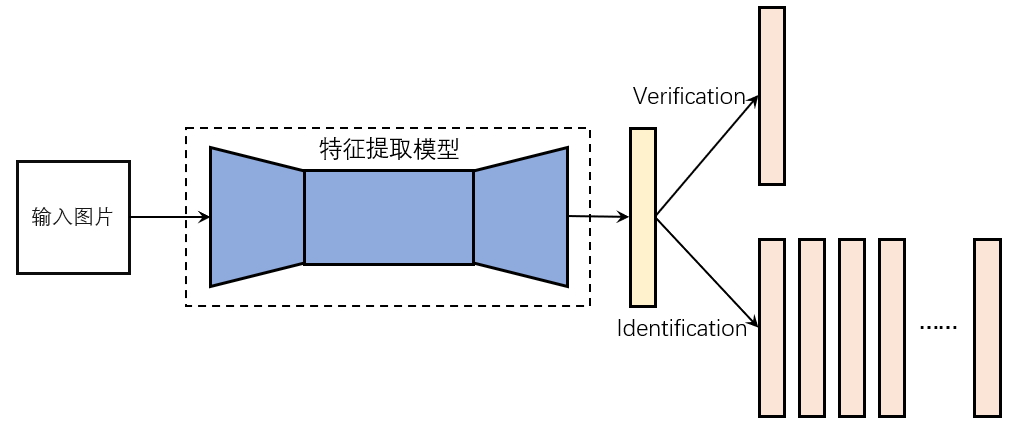
\includegraphics[scale=0.55]{img/chapter_fr/verification_identification.png}
\caption{人脸特征抽取}
\label{fig:verification_identification}
\end{figure}


传统的特征提取算法,通过一些降维方法,得到一系列降维后的特征,用来表示人脸。比如使用PCA进行降维的EigenFace,基于LDA进行降维的FisherFace等,都是早期人脸识别中非常经典的算法。但这些方法存在一些缺点,对光照、表情、姿态敏感,泛化能力不足,因此在实际使用中的准确度不高。

随着深度学习的广泛应用,越来越多具有实用价值的方法被提出,人脸识别的研究得到了极大的发展。基于深度学习的特征提取方法可以分为两大类:
\paragraph{度量学习(metric learning)}
通过一个度量函数,来衡量相同人或者不同人的特征表示之间的距离,从而学习到每个人每个照片的特征表示,基本思路是同一个人的特征表示之间的距离尽可能小,不同人的特征表示的距离尽可能大。
这一个方向的典型方法包含2014年的Contrastive loss\cite{sun2014deep}和2015年google提出的Triplet loss\cite{schroff2015facenet}。

DeepID2是基于Contrastive loss的模型,它在训练的时候,同时训练classification和verification两个信号,其中的verification信号,就是用特征表示之间的Contrastive loss来构造的。Contrastive loss是基于pairwise的思想,模型训练时,需要输入两张图片,如果两个图片是同一个人,则verification的标签为1,如果不是同一个人,则标签为0。

google于2015年提出的Facenet中,则用到了Triplet loss。其思想是以三元组的形式来训练模型,每次输入需要三张图片,其中两张图片是同一个人,以及一张其他人的图片,要求同一个人的照片之间的距离要小于不同人之间的距离,且要超过一个margin。具体公式如下所示:
\[L_{triplet}=\sum_{i=1}^{N}max\{0, \parallel f(x_i^a) - f(x_i^p) \parallel_2^2 - \parallel f(x_i^a) - f(x_i^n) \parallel_2^2 + \alpha \}\]
其中,$f(\cdot)$表示输入图像的特征表示,$x_i^a$表示anchor样本,$x_i^p$表示positive样本,$x_i^n$表示negative样本,$\alpha$表示对应的margin。

\paragraph{基于margin的分类方法(margin based classification)}
第二类思想是基于分类的思想来进行特征提取,根据训练集中的数据,同一个人的照片属于同一类,训练集一共包含多少个id,则总共需要分多少类。由于用的分类的思想,所以自然而然可以使用分类的损失函数。而在此基础上,又提出了一系列的方法,用以最小化类内间距或者最大化类间间距。比较有代表性的方法有Center loss\cite{wen2016discriminative},SphereFace\cite{liu2017sphereface},CosFace\cite{wang2018cosface}以及ArcFace\cite{deng2019arcface}等。

由于是多分类任务,所以最基本的损失函数形式是softmax loss,softmax loss是指概率输出函数为softmax函数,且损失函数为交叉熵(cross entropy)。但是直接用softmax loss训练出来的特征,往往效果不理想,某些类别的类内间距甚至比类间间距大,导致人脸识别的时候出现错误。center loss引入了类内中心,为每个类别提供一个类内中心,最小化训练集中每个样本与其类内中心的距离,从而达到减少类内间距的效果。具体形式如下所示:
\begin{equation*}
\begin{split}
L_{centerloss}&=L_S + \lambda L_C \\
&=-\frac{1}{N}(\sum_{i=1}^{N}log(\frac{e^{W_{y_i}^T f(x_i) + b_{y_i}}}{\sum_{j=1}e^{W_j^T f(x_i) + b_j}}) + \frac{\lambda}{2}\sum_{i=1}^{N}\parallel f(x_i) - c_{y_i}\parallel_2^2) \\
\end{split}
\end{equation*}
其中,$c_{y_i}$表示$x_i$所对应类别的中心,它与$f_(x_i)$的维度一致,该类别中心与参数一样,需要在训练中迭代更新。

基于SphereFace的训练方式,是在此基础上做了改进,对权重进行了归一化,且增加了角度裕量,在cos函数上对角度乘上因子m,加大分类难度。具体形式如下所示:
\[L_{sphereface}=-\frac{1}{N}\sum_{i=1}^{N}log(\frac{e^{{\parallel f(x_i) \parallel_2}cos(m\theta_{y_i,i})}}{e^{{\parallel f(x_i) \parallel_2}cos(m\theta_{y_i,i})} + \sum_{j \ne y_i}e^{{\parallel f(x_i) \parallel_2}cos(\theta_{j,i})}})\]

CosFace和ArcFace更进一步,对特征$f(x_i)$也做了归一化,并分别引入了不同的margin形式,取得了更好的效果,如下所示:
\[L_{cosface}=-\frac{1}{N}\sum_{i=1}^{N}log(\frac{e^{s(cos(\theta_{y_i, i})-m)}}{e^{s(cos(\theta_{y_i, i})-m)} + \sum_{j \ne y_i} e^{s cos(\theta_{j,i})}})\]

\[L_{arcface}=-\frac{1}{N}\sum_{i=1}^{N}log(\frac{e^{s cos(\theta_{y_i, i} + m)}}{e^{s cos(\theta_{y_i, i} + m)} + \sum_{j \ne y_i} e^{s cos(\theta_{j,i})}})\]

以上方法都是通过不同方式去减少同一个人的类内间距以及增大不同人之间的类间间距。但除了损失函数以及网络的设计之外,更为重要的是训练的数据的分布,比较好的训练数据是同一个人包含多张不同的照片,这些照片覆盖此人不同年龄段,不同姿态角度,不同遮挡程度,不同妆容情况等,这样的数据能够学习到鲁棒性更强,通用性更好的模型。
\section{应用案例}

人脸识别目前在安防、金融等领域都得到了广泛应用,下面介绍一些常见的应用案例。
\paragraph{门禁闸机}
这是人脸识别的典型应用场景,属于人脸检索(1:N)的应用。门禁闸机在初始化的时候,会要求录入一个人脸库,该人脸库经过特征提取后,作为识别的底库。当有人通过闸机的时候,会拍摄来人的照片,通过特征提取转化为特征表示之后,与底库中的特征集合进行对比,找出该人员是否存在于底库中。
\paragraph{金融核身业务}
目前几乎所有的金融核身业务都支持人脸核身功能,属于人脸比对(1:1)的应用。当用户的办理某些业务的时候,会被要求进行人脸核身,系统会通过摄像头采集用户的照片,与用户留底的另一张照片进行比对,以确定用户是否为本人。这种方式大大减少了金融业务中进行业务审核的人员数量及审核时间,节省了用户时间,提升了用户体验。

\paragraph{监控系统}
在银行、机场、商场等公共场景对人群进行监控,这种场景属于非配合式场景,用户大多数情况下并不知道有摄像头在拍摄,不会对拍摄做出配合。因此此类场景的拍摄距离通常会较远,用户姿态多样,且可能会有各种遮挡问题。相比于上面两种应用场景,此类场景较复杂,技术难度也较高。这种场景下,除了对监控中的人进行人脸检索外,还可能会进行人脸属性识别,如识别人的年龄,性别等,以便于后续进行更细致的分析。